\documentclass[border=5mm]{standalone}
\usepackage{pgfplots}
\pgfplotsset{compat=1.18}

\begin{document}
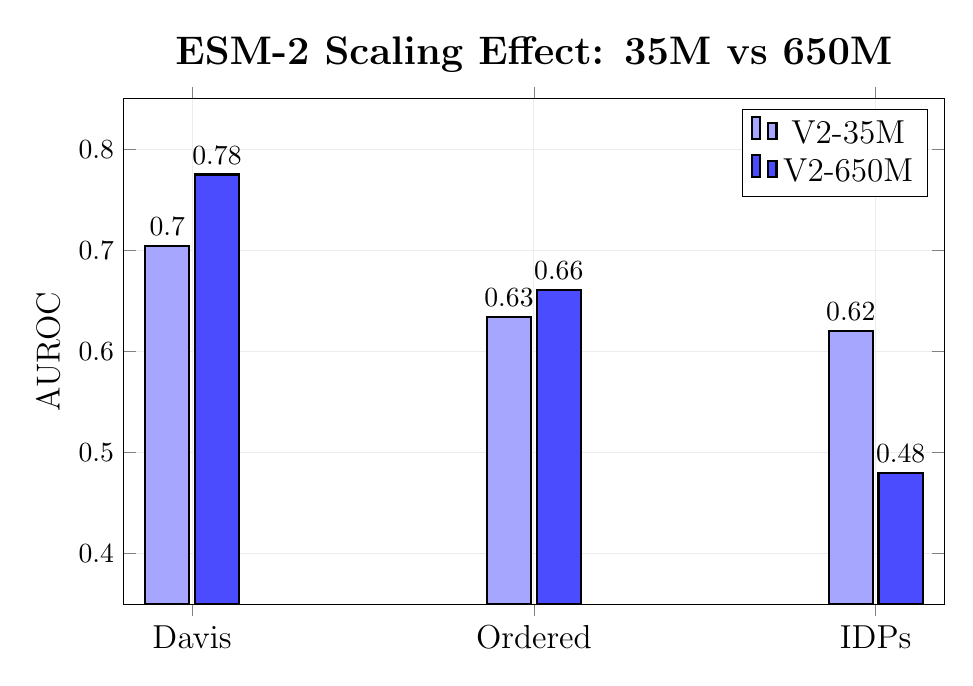
\begin{tikzpicture}
\begin{axis}[
    ybar,
    bar width=16pt,
    width=12cm,
    height=8cm,
    ylabel={AUROC},
    ylabel style={font=\large},
    symbolic x coords={Davis, Ordered, IDPs},
    xtick=data,
    x tick label style={font=\large},
    ymin=0.35, ymax=0.85,
    title={\textbf{ESM-2 Scaling Effect: 35M vs 650M}},
    title style={font=\Large},
    legend style={at={(0.98,0.98)}, anchor=north east, font=\large},
    nodes near coords,
    nodes near coords style={font=\normalsize, anchor=south},
    grid=major,
    grid style={gray!15},
    ymajorgrids=true,
    every axis plot/.append style={thick},
]

\addplot[fill=blue!35] coordinates {(Davis, 0.704) (Ordered, 0.634) (IDPs, 0.620)};
\addplot[fill=blue!70] coordinates {(Davis, 0.775) (Ordered, 0.661) (IDPs, 0.480)};

\legend{V2-35M, V2-650M}

\end{axis}
\end{tikzpicture}
\end{document}
